\icode{N21J-ME-SI-L2-261017-002}
\nceeID[4]{2021河北}{6}
一半径为\(R\)的圆柱体水平固定，横截面如图所示。长度为\(\pi R\)、不可伸长的轻细绳，一端固定在圆柱体最高点\(P\)处，另一端系一个小球。小球位于\(P\)点右侧同一水平高度的\(Q\)点时，绳刚好拉直。将小球从\(Q\)点由静止释放，当与圆柱体未接触部分的细绳竖直时，小球的速度大小为（重力加速度为\(g\)，不计空气阻力）\paren[]

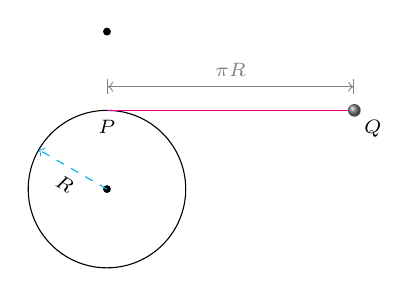
\begin{tikzpicture}[font=\scriptsize]
	\draw (0,0) circle(1);
	\draw[magenta] (0,1)node[below,black]{\(P\)}--({pi},1)node[below right,black]{\(Q\)};
	\shade[ball color=gray] ({pi},1) circle(.08);
	\draw[|<->|,gray] (0,1.3)--node[above]{\(\pi R\)}({pi},1.3);
	\fill (0,2) circle(.05);
	\fill (0,0) circle(.05);
	\draw[->,dashed,cyan] (0,0)--node[below,rotate=-30,black]{\(R\)}(150:1);
\end{tikzpicture}
\begin{choices}
	\item \(\sqrt{(2 +\pi)gR}\)
	\item \(\sqrt{2\pi gR}\)
	\item \(\sqrt{2(1 +\pi)gR}\)
	\item \(2\sqrt{gR}\)
\end{choices}
\begin{answer}
	A\qquad 提示：注意计算小球下落高度
\end{answer}